% !TeX root = ../main.tex
\section{Real-Flight Effective-Wrench Dataset}
\label{sec:dataset}

\subsection{Flight Platform and Onboard Logging}
\label{subsec:platform_logging}

The dataset was collected on a bird-scale flapping-wing vehicle designed for outdoor autonomous forward flight. Table~\ref{tab:platform_params} summarizes the platform, sensing, and logging quantities that are used later for effective-wrench reconstruction and residual modeling, and Fig.~\ref{fig:platform_dataset} shows the vehicle during flight. The vehicle mass and geometry set the scale of the reconstructed force and moment labels, while the logging configuration determines which state, actuation, airdata, and wingbeat variables are available to the causal model.

\begin{table}[t]
\caption{Platform and onboard logging summary for the flapping-wing vehicle.}
\label{tab:platform_params}
\centering
\resizebox{\columnwidth}{!}{%
\begin{tabular}{@{}ll@{}}
\toprule
Item & Value or role \\
\midrule
Nominal takeoff mass & $\approx 0.95~\mathrm{kg}$; three-point weighing value \needinfo{TBD} \\
Wingspan & $1.6~\mathrm{m}$ \\
Flight speed range & $4$--$10~\mathrm{m/s}$ \\
Maximum flapping frequency & $6.8~\mathrm{Hz}$ \\
Flight controller & Pixhawk 6C Mini running PX4 fixed-wing stack \\
Primary lift/propulsion & Single main flapping mechanism \\
Tail effectors & Left/right horizontal tails and vertical tail \\
Airspeed sensing & Pitot-static probe with MS4525DO pressure sensor \\
Position sensing & RTK-capable GNSS absolute positioning \\
Wingbeat sensing & AS5600 encoder at $100~\mathrm{Hz}$ and Hall-indexed phase path \\
CG measurement & Plumb-line suspension; $\mathbf{r}_{\mathrm{CG}}$ \needinfo{TBD} \\
Inertia measurement & Bifilar-pendulum measurement; $\mathbf{I}_{B,\mathrm{CG}}$ \needinfo{TBD} \\
IMU-to-CG survey & Mechanical survey used for reference-point alignment; $\mathbf{r}_{\mathrm{IMU}/\mathrm{CG}}^{B}$ \needinfo{TBD} \\
Actuator logging & \texttt{actuator\_motors} and \texttt{actuator\_servos}, binned to $100~\mathrm{Hz}$ \\
Low-rate context & Airdata, wind, GPS, status, and allocator topics with freshness masks \\
Canonical sample rate & $100~\mathrm{Hz}$ after offline resampling \\
\bottomrule
\end{tabular}%
}
\end{table}

\begin{figure}[t]
  \centering
  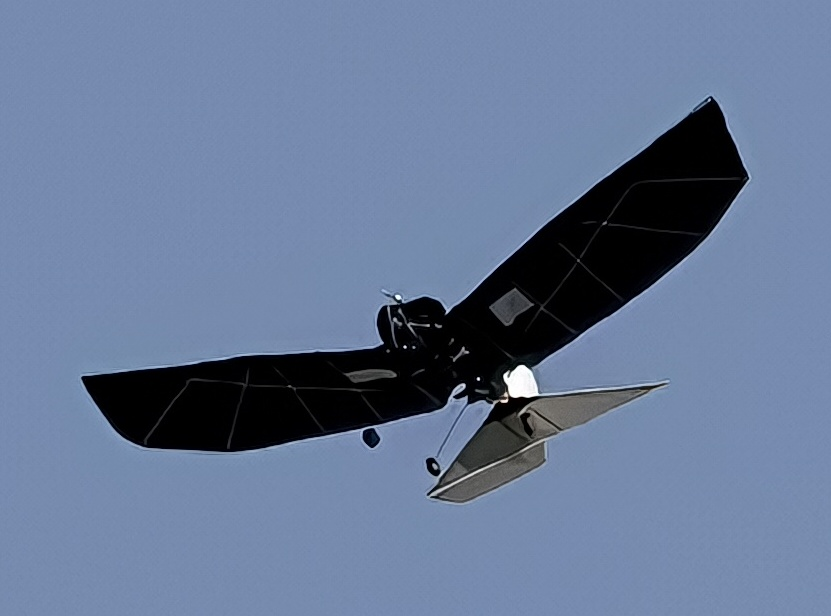
\includegraphics[width=0.98\columnwidth]{imgs/flying_img.jpg}
  \caption{Bird-scale flapping-wing vehicle during outdoor flight.}
  \label{fig:platform_dataset}
\end{figure}

The airframe uses a single motor-driven flapping mechanism to drive the two main wings and generate the dominant lift and propulsive force during forward flight. Attitude control is provided by three movable tail surfaces: the left and right horizontal tails act as elevon-like pitch and roll effectors, and the vertical tail provides yaw control. This actuation layout is important for the dataset definition because the reconstructed labels are not isolated wing loads. They are the net non-gravitational body-frame wrench that explains the measured rigid-body motion, including wing, tail, body, mechanism, and disturbance effects that are not separable from onboard logs alone.

The rigid-body quantities used in the wrench reconstruction are measured independently from the training logs. The vehicle mass is obtained with a three-point weighing setup, the center of gravity is located by a plumb-line suspension procedure, and the body-frame inertia matrix is obtained with a bifilar-pendulum measurement about the measured center of gravity. The measured values used in the final reconstruction are \needinfo{$m=\mathrm{TBD}~\mathrm{kg}$}, \needinfo{$\mathbf{r}_{\mathrm{CG}}=\mathrm{TBD}$}, and \needinfo{$\mathbf{I}_{B,\mathrm{CG}}=\mathrm{TBD}~\mathrm{kg\,m^2}$}. These bench measurements define the reference point used later for both the log-derived effective wrench and the simulator-prior wrench.

The onboard controller uses a PX4-based fixed-wing stack~\cite{meier2015px4}. In this configuration, the fixed-wing propulsion command is mapped to the flapping motor command, while the attitude and rate controllers command the three tail surfaces through the fixed-wing control-allocation path. The modeling dataset uses the resulting normalized outputs recorded in \texttt{actuator\_motors} and \texttt{actuator\_servos}; it does not require a detailed model of the guidance or mission controller.

The sensor and logging chain combines standard flight-state topics with flapping-specific measurements. The inertial estimator provides attitude, local velocity, local acceleration, angular velocity, and angular acceleration fields. RTK-capable GNSS and airdata topics provide outdoor flight context, including airspeed, density, and wind estimates. The flapping mechanism is measured with an AS5600 magnetic encoder, a Hall index pulse path, flapping-frequency and RPM topics, and, for the current paper split, a logged \texttt{wing\_phase} topic. The firmware also records encoder-count, Hall-event, flapping-frequency, RPM, motor-actuator, and servo-actuator topics. The preprocessing pipeline can fall back to encoder-count-derived phase when \texttt{wing\_phase} is absent, but all rows in the materialized split used here report \texttt{phase\_source=wing\_phase}. Thus the phase input for this paper is Hall-indexed wing phase, followed by offline cycle correction for valid active wingbeats.

\subsection{Flight Logs and Operating Envelope}
\label{subsec:flight_logs_envelope}

The logs used in this paper come from outdoor mission and forward-flight segments rather than bench tests or wind-tunnel measurements. The raw ULogs are first converted to canonical samples, and the final training tables retain only rows that satisfy the dataset validity masks. In the materialized split, a row must have a valid effective-wrench label, a valid wingbeat cycle, active flapping, and a non-landed state. The split manifest also applies an altitude-window trim that keeps the continuous airborne interval above $5~\mathrm{m}$ altitude. These filters remove takeoff and landing transients, landed samples, invalid phase samples, invalid state samples, and rows for which the reconstructed label is not available. Mode, arming, and landed-state changes define segment boundaries, so temporal windows are not allowed to cross those discontinuities.

Table~\ref{tab:flight_campaign_summary} summarizes the flight campaign metadata associated with the retained logs. The retained samples correspond to $74.8~\mathrm{min}$ of valid $100~\mathrm{Hz}$ flight data after filtering. Table~\ref{tab:log_split_envelope} reports the log inventory and the operating envelope used for the paper, and Fig.~\ref{fig:operating_envelope} visualizes how the retained samples are distributed across the same flight-condition variables. The split is whole-log: each flight log is assigned entirely to training, validation, or test. The date distribution is not identical across splits because logs are kept intact, but every split contains held-out logs from multiple flight days. The envelope statistics are reported as 5th, 50th, and 95th percentiles over all retained samples, which is more informative than the raw extrema because low-rate airdata and outdoor wind estimates can contain occasional edge values even after freshness filtering.

\begin{table*}[t]
\caption{Flight-campaign summary for the retained outdoor logs. Red entries mark campaign notes to be filled with field-test records before submission.}
\label{tab:flight_campaign_summary}
\centering
\resizebox{\textwidth}{!}{%
\begin{tabular}{@{}lrrrrl p{0.29\textwidth} p{0.22\textwidth}@{}}
\toprule
Date & Logs & Retained rows & Retained time [min] & Split use & Flight mode / trajectory & Campaign notes & Wind / weather record \\
\midrule
2026-4-12 & 3 & 49967 & 8.33 & Train/Val/Test & Outdoor forward-flight mission & \needinfo{TBD: waypoint/loiter/straight-segment description, altitude band, pilot/autonomy mode} & \needinfo{TBD: surface wind, logged wind summary, temperature} \\
2026-4-14 & 6 & 108974 & 18.16 & Train/Val/Test & Outdoor forward-flight mission & \needinfo{TBD: waypoint/loiter/straight-segment description, altitude band, pilot/autonomy mode} & \needinfo{TBD: surface wind, logged wind summary, temperature} \\
2026-4-15 & 10 & 150943 & 25.16 & Train/Val/Test & Outdoor forward-flight mission & \needinfo{TBD: waypoint/loiter/straight-segment description, altitude band, pilot/autonomy mode} & \needinfo{TBD: surface wind, logged wind summary, temperature} \\
2026-4-16 & 10 & 139076 & 23.18 & Train/Val/Test & Outdoor forward-flight mission & \needinfo{TBD: waypoint/loiter/straight-segment description, altitude band, pilot/autonomy mode} & \needinfo{TBD: surface wind, logged wind summary, temperature} \\
\midrule
Total & 29 & 448960 & 74.83 & Train/Val/Test & -- & -- & -- \\
\bottomrule
\end{tabular}%
}
\end{table*}

\begin{table}[t]
\caption{Whole-log split and retained operating envelope. The first panel gives log/sample counts by flight date and split. The second panel gives percentiles over all retained samples in the 29-log paper split.}
\label{tab:log_split_envelope}
\centering
\resizebox{\columnwidth}{!}{%
\begin{tabular}{@{}lrrrrrr@{}}
\toprule
Date & Train logs & Val logs & Test logs & Train rows & Val rows & Test rows \\
\midrule
2026-4-12 & 1 & 1 & 1 & 14208 & 17575 & 18184 \\
2026-4-14 & 4 & 1 & 1 & 77576 & 17187 & 14211 \\
2026-4-15 & 7 & 2 & 1 & 105461 & 31280 & 14202 \\
2026-4-16 & 8 & 1 & 1 & 111457 & 13545 & 14074 \\
\midrule
Total & 20 & 5 & 4 & 308702 & 79587 & 60671 \\
\bottomrule
\end{tabular}%
}
\vspace{0.4em}
\resizebox{\columnwidth}{!}{%
\begin{tabular}{@{}lccc@{}}
\toprule
Quantity & 5th percentile & Median & 95th percentile \\
\midrule
True airspeed $[\mathrm{m/s}]$ & 5.15 & 8.20 & 10.23 \\
Angle of attack $[\mathrm{deg}]$ & 11.57 & 20.40 & 28.30 \\
Sideslip $[\mathrm{deg}]$ & -11.56 & -1.59 & 9.24 \\
Cycle flapping frequency $[\mathrm{Hz}]$ & 3.49 & 4.35 & 4.91 \\
Dynamic pressure $[\mathrm{Pa}]$ & 15.19 & 38.29 & 59.53 \\
\bottomrule
\end{tabular}%
}
\end{table}

\begin{figure*}[t]
  \centering
  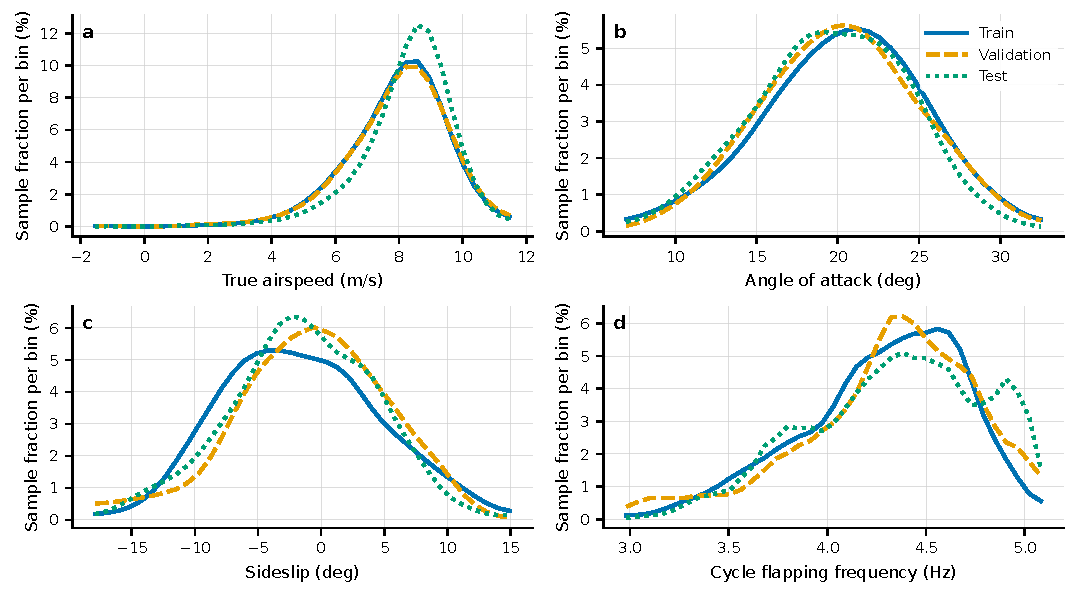
\includegraphics[width=0.88\textwidth]{figures/operating_envelope_summary.pdf}
  \caption{Operating-envelope distributions after preprocessing and whole-log splitting. Each panel shows lightly smoothed sample-fraction curves computed from common bins for true airspeed, angle of attack, sideslip, and cycle flapping frequency, using the retained samples from the training, validation, and test logs. The figure defines the flight-condition range for the log-based evaluation; it is not a closed-loop simulation or controller-performance result.}
  \label{fig:operating_envelope}
\end{figure*}

The purpose of these statistics is to define the evaluation boundary. The held-out metrics in Sec.~\ref{sec:results} measure interpolation and cross-log generalization within this retained outdoor envelope. They do not show performance for takeoff, landing, aggressive maneuvers outside the logged range, or closed-loop simulation with the learned residual model.

\subsection{Effective-Wrench Reconstruction}
\label{subsec:wrench_target}

\begin{figure}[t]
  \centering
  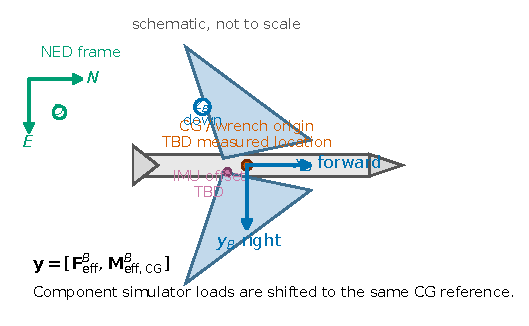
\includegraphics[width=0.98\columnwidth]{figures/wrench_reference_schematic.pdf}
  \caption{Schematic reference definition for effective-wrench reconstruction. The body frame follows forward-right-down convention and is attached to the measured center of gravity. Both the log-derived effective wrench and the simulator-prior wrench are expressed in this frame and reported about the same CG reference point. Red labels mark measured metadata values to be filled in the final draft.}
  \label{fig:wrench_reference}
\end{figure}

The target contains the three body-frame force components and the three body-frame moment components, using the reference convention summarized in Fig.~\ref{fig:wrench_reference}. We refer to this six-component vector as an effective wrench and write it as
\begin{equation}
  \mathbf{y}_t =
  \begin{bmatrix}
  f_{x,b} & f_{y,b} & f_{z,b} & m_{x,b} & m_{y,b} & m_{z,b}
  \end{bmatrix}^{\mathsf{T}},
  \label{eq:wrench_vector}
\end{equation}
where the body frame $B$ follows the forward-right-down convention, its origin is the measured center of gravity, and the navigation frame $N$ follows the north-east-down convention. The word effective is deliberate. The label is the net non-gravitational external wrench, about the measured CG, required to explain the measured rigid-body motion; it is not a direct wind-tunnel measurement of pure aerodynamic force and moment. It may include flapping-wing aerodynamics, tail and body aerodynamics, mechanism reaction effects, airdata and state-estimation errors, and outdoor disturbances.

The effective force is reconstructed from the translational dynamics. With $\mathbf{R}_{BN}$ denoting the rotation from navigation coordinates to body coordinates,
\begin{equation}
  \mathbf{F}_{\mathrm{eff}}^{B}
  =
  m\,\mathbf{R}_{BN}
  \left(
    \mathbf{a}^{N} - \mathbf{g}^{N}
  \right),
  \label{eq:force_label}
\end{equation}
where $m$ is the vehicle mass, $\mathbf{a}^{N}$ is the local-frame acceleration estimate, and $\mathbf{g}^{N}=[0,0,g]^{\mathsf{T}}$ in NED coordinates. The subtraction removes gravity before the result is expressed in body FRD coordinates, so upward lift appears as a negative $f_{z,b}$ component.

The effective moment is reconstructed from rigid-body rotational dynamics,
\begin{equation}
  \mathbf{M}_{\mathrm{eff}}^{B}
  =
  \mathbf{I}_{B}\boldsymbol{\alpha}_{B}
  +
  \boldsymbol{\omega}_{B}
  \times
  \left(
    \mathbf{I}_{B}\boldsymbol{\omega}_{B}
  \right),
  \label{eq:moment_label}
\end{equation}
where $\mathbf{I}_{B}$ is the body-frame inertia matrix about the measured CG, $\boldsymbol{\omega}_{B}$ is the body angular velocity, and $\boldsymbol{\alpha}_{B}$ is the body angular acceleration. In the current canonical pipeline, $\boldsymbol{\alpha}_{B}$ is read from the PX4 angular-velocity derivative fields; a smoothed-derivative path is also used for the sensitivity check reported later. The rigid-body metadata supplied to Eqs.~\eqref{eq:force_label}--\eqref{eq:moment_label} are \needinfo{$m=\mathrm{TBD}~\mathrm{kg}$}, \needinfo{$\mathbf{r}_{\mathrm{CG}}=\mathrm{TBD}$}, \needinfo{$\mathbf{r}_{\mathrm{IMU}/\mathrm{CG}}^{B}=\mathrm{TBD}$}, and \needinfo{$\mathbf{I}_{B,\mathrm{CG}}=\mathrm{TBD}~\mathrm{kg\,m^2}$}. These values are obtained from the three-point weighing, plumb-line CG, mechanical offset survey, and bifilar-pendulum inertia procedures described above.

The same reference point is used when comparing the log-derived wrench with the DeLaurier-style simulator prior. If the prior computes component loads at wing, tail, fuselage, or body reference points, each component is shifted to the measured CG before summation:
\begin{equation}
  \mathbf{M}_{\mathrm{sim,CG}}^{B}
  =
  \sum_j
  \left(
    \mathbf{M}_{j}^{B}
    +
    \mathbf{r}_{j/\mathrm{CG}}^{B}
    \times
    \mathbf{F}_{j}^{B}
  \right),
  \label{eq:sim_wrench_reference_shift}
\end{equation}
where $\mathbf{r}_{j/\mathrm{CG}}^{B}$ points from the measured CG to the component load reference. This alignment prevents a moment residual from being created purely by comparing two wrenches about different points. The component reference locations used for the final prior are \needinfo{TBD: wing, tail, fuselage, and body load-reference coordinates}.

\begin{table*}[t]
\caption{Main error sources in log-based effective-wrench labels and the associated checks used to bound them. Red entries mark numerical values to be filled with the final measurement and sensitivity results.}
\label{tab:wrench_error_sources}
\centering
\resizebox{\textwidth}{!}{%
\begin{tabular}{@{}p{0.18\textwidth}p{0.45\textwidth}p{0.28\textwidth}@{}}
\toprule
Source & How it enters the reconstructed label & Measurement or sensitivity record \\
\midrule
Acceleration noise & Directly changes $\mathbf{F}_{\mathrm{eff}}^{B}$ after gravity compensation. & Force-label smoothing sensitivity \needinfo{TBD: filter/window and force RMSE or label variation}. \\
Attitude error & Rotates both gravity-compensated acceleration and derived air-relative quantities. & Estimator quality and attitude innovation summary \needinfo{TBD}. \\
Rate and acceleration differentiation & Affects $\boldsymbol{\alpha}_{B}$ and therefore the moment label. & Angular-acceleration smoothing sensitivity \needinfo{TBD: moment-label variation and selected derivative path}. \\
Time alignment & Misaligns state, actuation, airdata, and phase at wingbeat time scales. & Topic age limits and phase-alignment check \needinfo{TBD: maximum age / phase delay tolerance}. \\
Mass, inertia, and CG uncertainty & Scales force and moment and changes the moment reference assumptions. & Three-point weighing, plumb-line CG, and bifilar-pendulum inertia; perturbation sensitivity \needinfo{TBD: mass, CG offset, inertia ranges}. \\
Reference-point mismatch & Creates artificial moment residuals when component loads and reconstructed moments are not expressed about the same point. & All prior component loads shifted to measured CG using Eq.~\eqref{eq:sim_wrench_reference_shift}; component coordinates \needinfo{TBD}. \\
Unmodeled mechanism reaction & Appears in the effective wrench but is not separable from aerodynamic load. & Treated as part of effective wrench; mechanism-state diagnostic \needinfo{TBD if included}. \\
Airdata and wind estimation & Affects model inputs and flight-condition interpretation. & Logged airdata and wind freshness plus campaign weather record \needinfo{TBD}. \\
Sensor freshness & Low-rate airdata, wind, GPS, and status topics are held with age masks. & Freshness thresholds and retained-valid fraction \needinfo{TBD}. \\
\bottomrule
\end{tabular}%
}
\end{table*}

These errors enter the supervised target itself. Consequently, the residual analyzed later should not be interpreted as one unique physical mechanism. It is a simulator-to-flight effective-wrench discrepancy under the sensing, metadata, and reconstruction assumptions above.

\subsection{Preprocessing, Model Inputs, and Whole-Log Split}
\label{subsec:canonical_samples}

Raw ULog topics are converted to a canonical $100~\mathrm{Hz}$ grid before model training. The preprocessing code constructs a uniform timeline from the core high-rate topics and then applies topic-specific resampling rules. Actuator motor and servo commands are averaged within each $10~\mathrm{ms}$ bin. Continuous states such as local position, velocity, acceleration, attitude quaternion components, angular velocity, and angular acceleration are linearly resampled on the grid, with quaternion normalization performed during downstream derived-feature construction. Low-rate airdata, wind, GPS, status, and allocator-status topics are held with zero-order hold and freshness masks. These freshness flags keep stale low-rate values identifiable instead of silently treating them as synchronous high-rate measurements.

Wingbeat phase is handled separately because it is central to the residual structure. The pipeline first reconstructs encoder and drive phase from encoder counts and metadata. If a fresh \texttt{wing\_phase} topic is present, as in the present paper split, that Hall-indexed phase becomes the raw phase source. The pipeline then annotates active flapping cycles, removes incomplete edge cycles, and maps each valid cycle to a corrected $[0,2\pi]$ phase coordinate. The final retained rows therefore satisfy \texttt{flap\_active}, \texttt{cycle\_valid}, and \texttt{label\_valid}. This filtering is why the sample counts in Table~\ref{tab:log_split_envelope} are lower than the raw ULog row counts.

The model inputs are organized into four groups. The state group contains attitude-derived quantities, body angular velocity, local and body-frame velocities, gravity direction, and air-relative velocity quantities such as angle of attack and sideslip. The actuation group contains the flapping motor command and the three tail-surface commands, including elevator-like and aileron-like combinations of the horizontal-tail pair. The flapping group contains corrected phase, phase sine and cosine, wing-stroke angle, flapping frequency, and cycle-level flapping frequency. The airdata group contains measured airspeed, air density, dynamic pressure, and wind estimates. These groups are used both for memoryless baselines and for causal temporal models, where phase, actuation, and airdata histories are allowed while current-state quantities are provided only at the prediction time.

The input design enforces a causal reconstruction boundary. Translational acceleration, angular acceleration, and past wrench targets are not provided as neural-model inputs in the paper feature set; acceleration is used only to reconstruct Eq.~\eqref{eq:force_label}, and angular acceleration is used only in Eq.~\eqref{eq:moment_label}. This prevents the network from learning the label by reading the same acceleration channels used to define it.

Finally, the dataset is split at the whole-log level to avoid temporal leakage. Splitting one flight log across training and testing would place nearby samples with similar phase, actuator history, airdata, wind condition, estimator history, and airframe condition in different sets. The current high-quality paper split therefore contains 29 logs: 20 training logs, 5 validation logs, and 4 test logs. The corresponding sample counts are 308702 training samples, 79587 validation samples, and 60671 test samples.
